\documentclass{amsart}
\usepackage{amsmath}
\usepackage{amsthm}
\usepackage{amssymb}

\usepackage{graphicx}

\usepackage{../../clontzDefinitions}

\newtheorem{theorem}{Theorem}[section]
\newtheorem{proposition}[theorem]{Proposition}
\newtheorem{lemma}[theorem]{Lemma}
\newtheorem{corollary}[theorem]{Corollary}


\theoremstyle{definition}
\newtheorem{definition}[theorem]{Definition}
\newtheorem{game}[theorem]{Game}
\newtheorem{example}[theorem]{Example}
\newtheorem{question}[theorem]{Question}



\begin{document}

% \title{Proximal compact spaces are Corson compact\tnoteref{t1}}
% \tnotetext[t1]{2010 Mathematics Subject Classification. 54E15, 54D30, 54A20.}
\title{On $k$-tactics in Gruenhage's compact-point game}

% \author[aub]{S.~Clontz\fnref{fn1}}
% \ead{steven.clontz@auburn.edu}
% \author[aub]{G.~Gruenhage\fnref{fn2}}
% \ead{gruengf@auburn.edu}

% \address[aub]{Department of Mathematics, Auburn University,
%  Auburn, AL 36830}


\author{Steven Clontz}
\address{Department of Mathematics, Auburn University,
Auburn, AL 36830}
\email{steven.clontz@gmail.edu}
\urladdr{www.stevenclontz.com}

\keywords{topological game, limited information strategy, metacompact spaces,
$\sigma$-metacompact spaces}

\subjclass[2010]{54D20, 54D45}


\begin{abstract}
Gary Gruenhage showed in \cite{MR858337} that metacompactness and
$\sigma$-metacompactness may be characterized for locally compact spaces
by way of a certain topological game using limited information strategies
which consider only the most recent move of the opponent (tactical/stationary
strategies) and possibly the round number (Markov strategies). This paper
demonstrates a non-trivial example of a space for which a winning strategy
exists but every limited information strategy considering a maximum of $k$
moves of the opponent and the round number may be defeated. The question
follows: are metacompactness and $\sigma$-metacompactness characterized by
winning $k$-tactical and $k$-Markov strategies?
\end{abstract}


\maketitle

\section{Introduction}

Consider the following topological game.

\begin{game}
  Let $\gruKPGame{X}$ denote the \term{Gruenhage compact/point game}
  with players $\pl K$, $\pl P$. During round $n$, $\pl K$ chooses
  a compact subset $K_n$ of $X$, followed by $\pl P$ choosing a point
  $p_n\in X$ such that $p_n\not\in \bigcup_{m\leq n}K_m$.

  $\pl K$ wins the game if the points $p_n$ are locally
  finite in the space, and $\pl P$ wins otherwise.
\end{game}

\begin{definition}
  A \term{strategy} for a game $G$ with moveset $M$ is a function
  $\sigma:M^{<\omega}\to M$; intuitively, this is a fixed rule for one player's
  choices in consideration of her opponent's moves. If using such a strategy
  always results in a win for the player $\pl P$ using it, then it is called a
  \term{winning strategy} and we write $\pl P\win G$.
\end{definition}

When $G(X)$ is a topological game played with space $X$, then $\pl P\win G(X)$
and $\pl P\not\win G(X)$ are topological properties of the space $X$.

The above game was used by the author's adviser Gary Gruenhage in
\cite{MR858337} to characterize
metacompactness (every open cover of the space has a point-finite open
refinement covering the space) and $\sigma$-metacompactness
(every open cover of the space has a $\sigma$-point-finite open refinement
covering the space) in locally compact spaces. However, the characterization
considers so-called \term{limited information strategies} which do not use
full information of the history of the game.

\begin{definition}
  A $k$-tactical strategy for a game $G$ with moveset $M$ is a function
  $\sigma:M^{\leq k}\to M$; intuitively, it is a strategy which only considers
  the previous $k$ moves of the opponent. If using such a strategy
  always results in a win for the player $\pl P$ using it, then
  we write $\pl P\ktactwin{k} G$.
\end{definition}

\begin{definition}
  A $k$-Markov strategy for a game $G$ with moveset $M$ is a function
  $\sigma:M^{\leq k}\times\omega\to M$; intuitively, it is a strategy which
  only considers the previous $k$ moves of the opponent and the round number.
  If using such a strategy
  always results in a win for the player $\pl P$ using it, then
  we write $\pl P\kmarkwin{k} G$.
\end{definition}

We will call $k$-tactical strategies ``$k$-tactics'' and $k$-Markov strategies
``$k$-marks''. If the $k$ is omitted then it is assumed that $k=1$. In
addition, note that some authors refer to tactics as
\term{stationary strategies}.

In this language, one may write Gruenhage's results as follows:

\begin{theorem}
  If $X$ is a locally compact space, then
  \begin{itemize}
    \item
    $X$ is metacompact if and only if $\pl K\tactwin\gruKPGame{X}$, and
    \item
    $X$ is $\sigma$-metacompact if and only if $\pl K\markwin\gruKPGame{X}$
  \end{itemize}
\end{theorem}

The main question essentially asks whether (at least for locally compact
spaces) a winning $(k+2)$-tactic or $(k+2)$-mark may always be improved to a
$1$-tactic or $1$-mark.

\begin{question}
  Let $X$ be a locally compact space and $k<\omega$.
  Does $\pl K\ktactwin{(k+2)}\gruKPGame{X}$ imply $X$ is metacompact?
  Does $\pl K\kmarkwin{(k+2)}\gruKPGame{X}$ imply $X$ is $\sigma$-metacompact?
\end{question}

This question is very similar to the open question on the well-known
Banach-Mazur (a.k.a. Choquet) game $\bmGame{X}$: does there exist a
space for which
$\pl N\ktactwin{3}\bmGame{X}$ but $\pl N\notktactwin{2}\bmGame{X}$
(where $\pl N$
is the player wishing for a nonempty intersection)?\footnote{
  The analogous question for $2$- and $1$-tactics was answered in the
  affirmative by Gabriel Debs in \cite{MR817083}.
}
For fans
of such infinite combinatorial game theory puzzles, we may restate the
main question as follows.

\begin{question}
  Does there exist a locally compact space $X$ such that
  $\pl K\ktactwin{2}\gruKPGame{X}$ but $\pl K\nottactwin\gruKPGame{X}$?
  What about for Markov strategies?
\end{question}


\section{Related results}

The game $\gruKPGame{X}$ has its roots in another topological game due to
Gruenhage.

\begin{game}
  Let $\gruConGame{X}{x}$ denote \term{Gruenhage's $W$-convergence game} with
  players $\pl O$, $\pl P$, for a topological space $X$ and point $x\in X$.
  In round $n$, $\pl O$ chooses an open neighborhood $O_n$ of $x$, followed
  by $\pl P$ choosing a point $p_n\in \bigcap_{m\leq n}O_m$.

  $\pl O$ wins the game if the points $p_n$ converge to $x$, and $\pl P$
  wins otherwise.
\end{game}

Let $\onePtComp{X}=X\cup\{\infty\}$ be the \term{one-point compactification}
of a noncompact locally compact space $X$, where points in $X$ have their
usual neighborhoods, and neighborhoods of $\infty$ are complements of
compact sets in $X$. Then convergence to $\infty$ in $\onePtComp{X}$
corresponds to local finiteness in the subspace $X$. One may then assume that
$\gruKPGame{X}$ and $\gruConGame{\onePtComp X}{\infty}$ are equivalent games
when $X$ is locally compact.
Considering perfect information, $1$-tactical, and $1$-Markov strategies, this
is essentially true.

\begin{theorem}
  If $X$ is locally compact, then
    \begin{itemize}
      \item $\pl K\win\gruKPGame{X}$ if and only if
        $\pl O\win\gruConGame{\onePtComp{X}}{\infty}$.
      \item $\pl K\markwin\gruKPGame{X}$ if and only if
        $\pl O\markwin\gruConGame{\onePtComp{X}}{\infty}$.
      \item $\pl K\tactwin\gruKPGame{X}$ if and only if
        $\pl O\tactwin\gruConGame{\onePtComp{X}}{\infty}$.
    \end{itemize}
\end{theorem}

\begin{proof}
  Let $\sigma$ be a winning mark for $\pl K$ in $\gruKPGame{X}$.
  Define the tactic $\tau$ for $\pl O$ in $\gruConGame{\onePtComp X}{\infty}$
  as follows:
    \[
      \tau(\emptyset,0) = \onePtComp{X}\setminus \sigma(\emptyset,0)
    \]
    \[
      \tau(\<x\>,n) =
        \left\{
          \begin{array}{lcr}
            \onePtComp{X} &
            : &
            x=\infty
              \\
            \onePtComp{X} \setminus \bigcup_{m\leq n}\sigma(\<x\>,m) &
            : &
            x\not=\infty
          \end{array}
        \right.
    \]
  Then for any legal attack $p$ against $\tau$, consider its subsequence
  $p'$ which removes all instances of $\infty$.
  If $p'$ is a finite sequence, then $p$ contains $\infty$ co-finitely and
  therefore converges to $\infty$.

  Note that for each $n<\omega$, $p'(n)=p(f(n))$ for some $f(n)\geq n$. Since
  $p$ is a legal attack against $\tau$,
    \[
      p'(n)
        =
      p(f(n))
        \in
      \tau(\emptyset,0)
        \cap
      \bigcap_{m<f(n)}\tau(\<p(m)\>,m+1)
    \]
    \[
        =
      \tau(\emptyset,0)
        \cap
      \bigcap_{m<n}\tau(\<p'(m)\>,f(m)+1)
        =
      \onePtComp{X}
        \setminus
      \left(
        \sigma(\emptyset,0)
          \cup
        \bigcup_{m<n,i\leq f(m)+1}\sigma(\<p'(m)\>,i)
      \right)
    \]
    \[
        \subseteq
      \onePtComp{X}
        \setminus
      \left(
        \sigma(\emptyset,0)
          \cup
        \bigcup_{m<n}\sigma(\<p'(m)\>,m+1)
      \right)
    \]
  so $p'$ is a legal attack against $\sigma$. Since $\sigma$ is a winning
  strategy, the points $p'(n)$ are locally finite in $X$, so
  $p'$ and therefore $p$ converge to $\infty$.

  If $\sigma$ is a winning mark for $\pl O$ in
  $\gruConGame{\onePtComp X}{\infty}$, let $\tau$ be a mark for
  $\pl K$ in $\gruKPGame{X}$ such that
    \[
      \tau(s,n) = X\setminus \sigma(s,n)
    \]
  Then for any legal attack $p$ against $\tau$, $p$ is a legal attack against
  $\sigma$. Since $\sigma$ is a winning
  strategy, $p$ converges to $\infty$,
  and therefore the points $p(n)$ are locally finite in $X$.

  The proofs of the first and third bullets are similar and are left to
  the reader.
\end{proof}

The reason why the games are not entirely equivalent is related to the extra
point $\infty$ in $\onePtComp X$, which gives $\pl P$ an extra choice in
$\gruConGame{\onePtComp X}{\infty}$ unavailable in $\gruKPGame{X}$.
In fact, a generalization of the above proof for a $(k+2)$-mark would not
hold.

For instance, suppose $\pl P$ wants to use a winning $2$-tactic $\sigma$ from
$\gruKPGame{X}$ to create a winning $2$-tactic for
$\gruConGame{\onePtComp X}{\infty}$. If $\pl P$ is attacked by
$\<x_0,\infty,x_2,\infty,\dots\>$, then $\pl P$ must ensure that the $x_{2n}$
converge without using the point $\infty\not\in X$.
It's difficult to see how, as $\pl P$ may not take advantage of
$\sigma(\<x_{2n},x_{2n+2}\>)$;
$x_{2n},x_{2n+2}$ are not consecutive moves in the original game.

So we cannot (at least easily) find a result for $\gruKPGame{X}$
comparable to the following result for $\gruConGame{X}{x}$:

\begin{proposition} For any $x\in X$ and $k<\omega$,
  \begin{itemize}
    \item
      $
      \pl O\ktactwin{(k+1)}\gruConGame{X}{x}
        \Leftrightarrow
      \pl O\tactwin\gruConGame{X}{x}
      $
    \item
      $
      \pl O\kmarkwin{(k+1)}\gruConGame{X}{x}
        \Leftrightarrow
      \pl O\markwin\gruConGame{X}{x}
      $
  \end{itemize}
\end{proposition}

\begin{proof}
  If $\sigma$ witnesses $\pl O\ktactwin{(k+1)}\gruConGame{X}{x}$,
  let $\tau(\emptyset)=\sigma(\emptyset)$ and
    \[
      \tau(\<p\>)
        =
      \bigcap_{i< k}
      \sigma(\<\underbrace{x,\dots,x}_{k-i},p,\underbrace{x,\dots,x}_{i+1}\>)
    \]

  Then $\tau$ is easily verified to be a winning tactic, and
  the proof for the second part is analogous.
\end{proof}

Note that this proof ironically relies on $\pl P$ playing
the point $x$ she wishes to avoid convergence to; a luxury not allowed to
$\pl P$ in $\gruKPGame{X}$ as that point ($\infty$) is fictional.

So we do have this corollary at least.

\begin{corollary}
  If $X$ is a locally compact space, then
  \begin{itemize}
    \item
    $X$ is metacompact if and only if
    $\pl K\tactwin\gruConGame{\onePtComp X}{\infty}$ if and only if
    $\pl K\ktactwin{(k+1)}\gruConGame{\onePtComp X}{\infty}$
    for some $k<\omega$, and
    \item
    $X$ is $\sigma$-metacompact if and only if
    $\pl K\markwin\gruConGame{\onePtComp X}{\infty}$ if and only if
    $\pl K\kmarkwin{(k+1)}\gruConGame{\onePtComp X}{\infty}$
    for some $k<\omega$.
  \end{itemize}
\end{corollary}


\section{A non-trivial example}

So if the analogous result does not hold for $\gruKPGame{X}$, then we
should be able to find a counterexample. Gruenhage suggested the following
class of spaces to the author:

\begin{definition}
  Let $\pmb X=(X\times 2^{<\omega})\cup C$ denote a Cantor tree
  of copies of a zero-dimensional, compact space $X$ with a point-countable
  cover $\mc{U} = \{U_\alpha : \alpha<\omega_1\}$ of distinct
  clopen sets, along with an uncountable subset of the Cantor set
  $C=\{c_\alpha:\alpha<\omega_1\}\in [2^\omega]^{\omega_1}$.
  The topology on $\pmb X$ is given by decaring $U\times\{s\}$ to be a open
  neighborhood of $\<x,s\>\in X\times 2^{<\omega}$ for each
  open neighborhood $U$ of $x$ in $X$, and declaring
  $
    B_{\alpha,m}
      =
    (U_\alpha\times\{c_\alpha\rest n: m\leq n<\omega\})\cup\{c_\alpha\}
  $
  to be a clopen neighborhood of $c_\alpha\in C$ for each $\alpha<\omega_1$,
  $m<\omega$.
\end{definition}

\begin{definition}
  Let $F\in \omega_1^{<\omega}$ and $m,n<\omega$.
  \[
    K_F = \bigcup_{\alpha \in F} B_{\alpha,0}
  \]
  \[
    a_n = \{\<i,0\>:i<n\}\cup\{\<n,1\>\}
  \]
  \[
    A = \{a_n : n<\omega\}
  \]
  \[
    K_F' = K_F \setminus (X \times A)
  \]
  \[
    L_m = X \times 2^{<m}
  \]
\end{definition}

Figure \ref{fig:pmbX} provides a rough illustration of
$\pmb X$, $L_m$ (the triangle at the base), and $K_F'$
(the branches of open sets descending from $C$).

\begin{figure}
  \centering
  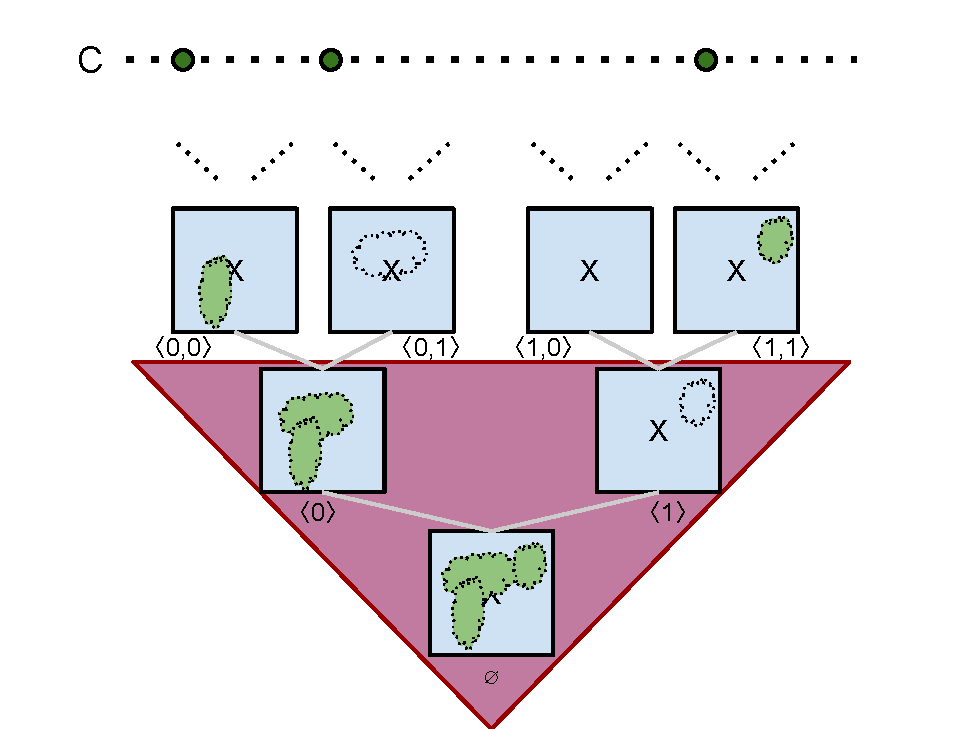
\includegraphics[width=\linewidth]{pmbX.pdf}
  \caption{$\pmb X$, with $L_m$ and $K_F'$}
  \label{fig:pmbX}
\end{figure}

\begin{lemma}
  $K_F$, $K_F'$, and $L_m$ are compact in $\pmb X$.
  Furthermore, every compact set is contained in a union of $K_F'$, $L_m$
  for some $F\in C^{<\omega}$ and $m<\omega$.
\end{lemma}

\begin{proof}
  $K_F$ contains $C_F=\{c_\alpha: \alpha\in F\}\subseteq C$, so any
  cover of basic open sets must include $B_{\alpha,n_\alpha}$ for each
  $\alpha\in F$, and the remaining uncovered portion of $K_F$ is a closed
  subset of a finite union of copies of compact $X$. Then $K_F'$ is also
  compact as it is a closed subset of $K_F$, and $L_m$ is compact as it
  is a finite union of copies of compact $X$.

  Let $D$ be compact. Consider the open cover
    \[
      \{
        B_{\alpha,0}
      :
        \alpha<\omega_1
      \}
      \cup
      \{
        X\times\{s\}
      :
        s\in 2^{<\omega}
      \}
    \]
  and note that the finite subcover for $D$ contains subsets of some
  $K_F' \cup L_m$.
\end{proof}

\begin{theorem}
  $\pl K\win\gruKPGame{\pmb X}$.
\end{theorem}

\begin{proof}
  Since $\{U_\alpha:\alpha<\omega_1\}$ is a point-countable cover,
  for each $x\in X$ let $\alpha_{x,n}<\omega_1$ yield
  ordinals such that $x\in U_{\alpha_{x,n}}$ for $n<\omega$.

  Let $M:\pmb X\times \omega\to \mc K(\pmb X)$ as follows:
    \[
      M(\pmb x,n)
        =
      \left\{
        \begin{array}{lcl}
          K_{\{\alpha_{x,m}:m\leq n\}}
        & : &
          \pmb x = \<x,s\> \in X\times 2^{<\omega}
        \\
          K_{\{\alpha\}}
        & : &
          \pmb x = c_\alpha \in C
        \end{array}
      \right.
    \]
  and use $M$ to define the strategy $\sigma$ for each
  $\pmb a\in\pmb X^{<\omega}$:
    \[
      \sigma(\pmb a)
        =
      L_{|\pmb a|}
        \cup
      \bigcup_{i< |\pmb a|}
      M(\pmb a(i),|\pmb a|)
    \]

  Let $\pmb p:\omega\to\pmb X$ be a legal attack against $\sigma$. Then as
  $\pmb p(n)\not\in L_n$, for each $\pmb x=\<x,s\>\in X\times 2^{<\omega}$,
  $X\times\{s\}$ is an open neighborhood of $\pmb x$ which contains finitely
  many $\pmb p(n)$.

  Now consider $\pmb x=c_\alpha$ for some $\alpha<\omega_1$, and let $n<\omega$.
  Then if $\pmb p(n)=\<x,s\>$ with $\alpha = \alpha_{x,N}$ for some $N<\omega$,
  then $\pmb p(m)\not\in B_{\alpha,0}$ for $\max(n,N)<m<\omega$.
  Or, if $\pmb p(n)=c_\alpha$, then
  $\pmb p(m)\not\in B_{\alpha,0}$ for $n<m<\omega$.
  Otherwise, $\pmb p(m)\not\in B_{\alpha,0}$ for any $m<\omega$.
  In any case, $B_{\alpha,0}$ is a neighborhood of $\pmb x$ which
  contains finitely
  many $\pmb p(n)$. Therefore, $\sigma$ is a winning strategy.
\end{proof}

One might hope then that $\pl K\nottactwin\gruKPGame{\pmb X}$ but
$\pl K\ktactwin{2}\gruKPGame{\pmb X}$, giving us our counterexample.
However, we will see that in fact, any winning $k$-mark for $\pl K$ may
be improved to a winning tactic by exploiting the structure of the Cantor tree.

In particular, knowledge of round number does not assist $\pl K$,
since she may force $\pl P$ to either stay within $C$, or to seed a growing
integer which could be used in place of the round number
by forcing her to play outside $L_{|s|+1}$ in response to
$\<x,s\>\in X\times 2^{<\omega}$.

\begin{lemma}
  If $\pl K\kmarkwin{(k+1)}\gruKPGame{\pmb X}$, then
  $\pl K\ktactwin{(k+1)}\gruKPGame{\pmb X}$.
\end{lemma}

\begin{proof}
  Let $\sigma$ be a winning $(k+1)$-mark for $\pl K$ such that $m\leq n$ and
  $\ran r \subseteq \ran s$ implies $\sigma(r,m)\subseteq\sigma(s,n)$.
  For a sequence $p$, let $p\rest^k n=\nu_k(p\rest n)$ give the last $k$
  terms of $p\rest n$.

  Define $r:\pmb X\to\omega$ by
    \[
      r(\pmb x)
        =
      \left\{
        \begin{array}{lcl}
          |s|
        & : &
          \pmb x = \<x,s\> \in X\times 2^{<\omega}
        \\
          0
        & : &
          \pmb x \in C
        \end{array}
      \right.
    \]
  and use $r$ to define the $(k+1)$-tactic $\tau$ by
    \[
      \tau(\emptyset)
        =
      \sigma(\emptyset,0)
    \]
    \[
      \tau(\pmb t\concat\<\pmb x\>)
        =
      L_{r(\pmb x)+1}
        \cup
      \{\pmb x\}
        \cup
      \sigma(\pmb t\concat\<\pmb x\>,r(\pmb x)+1)
    \]

  Let $\pmb p:\omega\to\pmb X$ be a legal attack by $\pl P$ against $\tau$.
  If $\pmb p(n)\in C$ for $N<n<\omega$, then since no $\pmb p(n)$ may be legally
  repeated, $\{\{\pmb p(n)\}:N<n<\omega\}$ is a discrete collection, making
  the points $p(n)$ locally finite.

  Otherwise, let $f\in\omega^\omega$ be increasing and define
  $\pmb q:\omega\to X\times 2^{<\omega}$ such that $\pmb q(i)=\pmb p(f(i))$,
  and $\pmb p(j)\in X\times 2^{<\omega}$ implies there is some $i$ with $j=f(i)$.
  It follows that
    \[
      \pmb q(0)
        =
      \pmb p(f(0))
        \not\in
      \bigcup_{m\leq f(0)}\tau(\pmb p \rest^{k+1} m)
        \supseteq
      \tau(\emptyset)
        =
      \sigma(\emptyset,0)
    \]

  Denoting $\pmb q(n)=\<x_n,s_n\>$, it's trivial to note that $|s_0|\geq 0$.
  Assuming that $|s_m|\geq m$ for $m\leq n$,
  it then follows that
    \[
      \pmb q(n+1)
        =
      \pmb p(f(n+1))
        \not\in
      \bigcup_{m\leq f(n+1)}\tau(\pmb p\rest^{k+1} m)
    \]
    \[
        \supseteq
      \bigcup_{m\leq n}\tau(\pmb q\rest^{k+1} m)
        \supseteq
      \sigma(\emptyset,0)
        \cup
      \bigcup_{m < n}\sigma(\pmb q\rest^{k+1} (m+1),|s_m|+1)
    \]
    \[
        \supseteq
      \sigma(\emptyset,0)
        \cup
      \bigcup_{m < n}\sigma(\pmb q\rest^{k+1} (m+1),m+1)
    \]
  and
    \[
      \pmb q(n+1)
        \not\in
      \tau(\pmb q\rest^{k+1} (n+1))
        \supseteq
      L_{r(\pmb q(n))}
        =
      L_{|s_n|+1}
    \]
  gives $|s_{n+1}|\geq|s_n|+1\geq n+1$.
  Thus $\pmb q$ is a legal attack on the winning $(k+1)$-Markov strategy
  $\sigma$, so the points $q(n)$ are locally finite,
  and it follows that the points $p(n)$ are also locally finite.
\end{proof}

\begin{corollary}
  $\pmb X$ is $\sigma$-metacompact if and only if $\pmb X$ is metacompact.
\end{corollary}

On the other hand, recalling a maximum of $k+1$ moves is only as good as
recalling the most recent move for $\pl K$, since $\pl P$ may always choose
to burn $k$ out of every $k+1$ moves
by moving down an antichain of the Cantor tree. Such movement would certainly
be locally finite (and therefore not directly benefit $\pl P$), but would
at least succeed in overloading $\pl K$'s limited memory.

\begin{lemma}
  If $\pl K\ktactwin{(k+1)}\gruKPGame{\pmb X}$, then
  $\pl K\tactwin\gruKPGame{\pmb X}$.
\end{lemma}

\begin{proof}
  Let $\sigma$ be a winning $(k+1)$-tactical strategy, and without loss of
  generality assume it ignores order.

  Define $F(x_0,\dots,x_{k},n)\in [C]^{<\omega}$ and
  $m(x_0,\dots,x_{k},n)\in\omega\setminus(n+1)$, both increasing on $n$,
  such that for each $\<x_0,\dots,x_{k}\>\in X^{k+1}$,
  \[
    \bigcup_{s_0,\dots,s_k \in 2^{\leq n}}
    \sigma(\<x_0,s_0\>,\dots,\<x_{k},s_{k}\>)
      \subseteq
    K'_{F(x_0,\dots,x_{k},n)} \cup L_{m(x_0,\dots,x_{k},n)}
  \]

  Select an arbitrary point $y \in X$.
  Let
    \[
      M^0(x,n)=n
    \]
    \[
      M^{i+1}(x,n)=m(x,y,\dots,y,M^i(x,n)+1)
    \]
  and define the tactical strategy $\tau$ as follows:
  \[
    \tau(\emptyset)
      =
    \sigma(\emptyset)
  \]
  \[
    \tau(\<c_\alpha\>)
      =
    \{c_\alpha\}
  \]
  \[
    \tau(\<\<x,s\>\>)
      =
    K'_{F(x,y,\dots,y,M^k(x,|s|)+1)}
      \cup
    L_{m(x,y,\dots,y,M^k(x,|s|)+1)}
  \]

  Let $\pmb p:\omega\to \pmb X$ be a legal attack against
  $\tau$, and assume $\pmb p(n)=\<x_n,s_n\>\in X\times 2^{<\omega}$.
  Then consider the attack $\pmb q:\omega\to X\times 2^{<\omega}$ against
  $\sigma$ defined by, for $n<\omega$ and $i<k$,
    \[
      \pmb q((k+1)n)=\pmb p(n)=\<x_n,s_n\>
    \]
    \[
      \pmb q((k+1)n+(i+1))=\<y, a_{M^{i+1}(x_n,|s_n|)}\>
    \]

  Since
    \[
      \<x_{n+1},s_{n+1}\>
        =
      \pmb p(n+1)
        \not\in
      \tau(\<\pmb p(n)\>)
        \supseteq
      L_{M^{k+1}(x_n,|s_n|)+1}
    \]
  it follows that
  $|s_{n+1}|\geq M^{i+1}(x_n,|s_n|)+1$ for $i<k$; furthermore,
    \[
      |s_n|
        \leq
      M^i(x_n,|s_n|)
        <
      M^i(x_n,|s_n|)+1
        \leq
      M^{i+1}(x_n,|s_n|)
        <
      M^{i+1}(x_n,|s_n|)+1
        \leq
      |s_{n+1}|
    \]
  so the second coordinate of $\pmb q(n)$ is always strictly increasing.

  By the definition of $\tau$,
    \[
      \pmb q((k+1)n)
        =
      \pmb p(n)
        \not\in
      \bigcup_{m\leq n}
      \tau(\pmb p\rest^1 m)
        \supseteq
      \bigcup_{m\leq (k+1)n}
      \sigma(\pmb q\rest^{k+1} m)
    \]

  Since
    \[
      \pmb q((k+1)n+(i+1))
        =
      \<y, a_{M^{i+1}(x_n,|s_n|)}\>
        \in
      X\times A
    \]
  it follows that $\pmb q((k+1)n+(i+1))\not\in K'_F$ for any
  $F\in[\omega_1]^{<\omega}$.

  Then it's sufficient to note that
    \[
      |a_{M^{i+1}(x_n,|s_n|)}|
        =
      M^{i+1}(x_n,|s_n|) + 1
        >
      m(x_n,y,\dots,y,M^i(x_n,|s_n|)+1)
    \]
  to show that
    \[
      \pmb q((k+1)n+(i+1))
        =
      \<y, a_{M^{i+1}(x_n,|s_n|)}\>
        \not\in
      L_{m(x_n,y,\dots,y,M^i(x_n,|s_n|)+1)}
    \]
  and therefore $\pmb q((k+1)n+(i+1))$ is a legal move.

  As a result, $\pmb q$ is a legal attack against $\sigma$, and
  $\{\{\pmb q(n)\}:n<\omega\}\supseteq\{\{\pmb p(n)\}:n<\omega\}$ are
  both locally finite.

  Finally, if the range of $\pmb p$ intersects $C$, those moves may be safely
  ignored as they cannot be repeated and lay in a closed discrete set,
  so the proof is complete.
\end{proof}

So our hopes for a counterexample to our main question
in $\pmb X$ are thusly defeated. Our
consolation prize will be to show that for a certain choice of $X$
and $\{U_\alpha:\alpha<\omega_1\}$, $\pmb X$ is at least
an example of a space which allows a winning strategy for $\gruKPGame{\pmb X}$
but no winning $k$-tactics or $k$-marks.

To this end, we will show that $\{U_\alpha:\alpha<\omega_1\}$ may be chosen
such that $\pmb X$ is not metacompact, and therefore
$\pl K$ lacks a $k$-Markov strategy for any $k<\omega$.

\begin{theorem}
  $\pmb X$ is metacompact
    if and only if
  $\{U_\alpha:\alpha<\omega_1\}$ is $\sigma$-point-finite.
\end{theorem}

\begin{proof}
  Let $\omega_1=\bigcup_{n<\omega}A_n$ such that
  $\{U_\alpha:\alpha\in A_n\}$ is point-finite for each $n<\omega$.

  Let $\mc U$ be a cover of $\pmb X$, and for each $s\in 2^\omega$
  let $\mc V_s$ be a finite open refinement of $\mc C$ covering the compact
  set $X\times\{s\}$. Then let $\mc W_n = \{B_{\alpha,n_\alpha}:\alpha\in A_n\}$
  be an open refinement of $\mc C$ for each $n<\omega$, and note that it
  is point-finite. It follows that
  $\mc U' = \bigcup_{s\in 2^{<\omega}} \mc V_s \cup \bigcup_{n<\omega} \mc W_n$
  is an open $\sigma$-point-finite refinement of $\mc U$, so $\pmb X$
  is $\sigma$-metacompact, and therefore it is metacompact.

  For the other direction, consider the open cover
  $\mc U = \{B_{\alpha,0}:\alpha<\omega_1\}$ of the closed subset $C$ of
  metacompact $\pmb X$, and let $\{B_{\alpha,n_\alpha}:\alpha<\omega_1\}$ be
  a point-finite refinement. Then
  $\mc U_s = \{ U_\alpha : c_\alpha \rest n_\alpha = s\}$ is
  point-finite for $s\in 2^{<\omega}$ and
  $U_\alpha\in\mc U_{c_\alpha\rest n_\alpha}$ for each $\alpha<\omega_1$.
  Therefore $\mc U = \bigcup_{s\in 2^{<\omega}} \mc U_s$ is
  $\sigma$-point-finite.
\end{proof}

\begin{theorem}
  There exists a compact, zero-dimensional topological space $X$
  with a clopen cover $\{U_\alpha : \alpha<\omega_1\}$ of distinct
  sets which is not $\sigma$-point-finite.
\end{theorem}

\begin{proof}
  Let $Y$ be a zero-dimensional Corson compact space which is not Eberlein
  compact; one such space was constructed in \cite{Marciszewski1991291}.
  Let $X=Y^2$.
  Then by characterizations of Corson and Eberlien compacts found in
  \cite{MR752278},
  $Y^2\setminus\Delta$ is meta-Lindel\"of but not $\sigma$-metacompact, so
  there exists a point-countable clopen cover $\mc U$ of $Y^2\setminus\Delta$
  which is not $\sigma$-point-finite. Then $\mc U\cup\{X\}$ is a point-countable
  clopen cover of $X$ which is not $\sigma$-point-finite.
\end{proof}

\begin{corollary}
  There exists a locally compact space $X$ such that $\pl K\win\gruKPGame{X}$
  but $\pl K\notkmarkwin{k} \gruKPGame{X}$ for all $k<\omega$.
\end{corollary}


\section{Acknowledgements}

The author would like to thank his PhD advisor Gary Gruenhage for his
support and mentorship while the author developed these results as a part of
his dissertation.


\bibliographystyle{plain}
\bibliography{../../bibliography}

\end{document}